\chapter{Introduction}
%JUSTIFICACION
\begin{figure}[b]
    \centering
    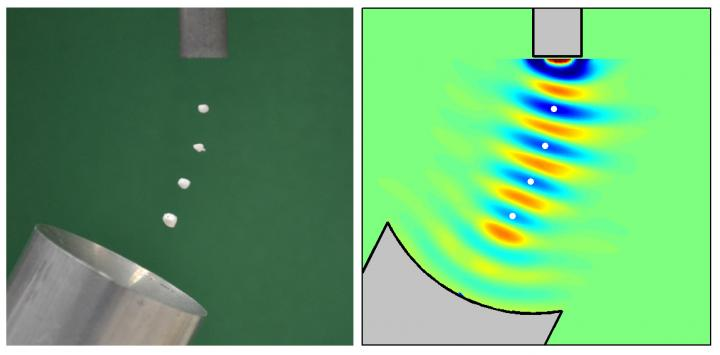
\includegraphics[width=0.45\textwidth]{images/intro/ac_levitaion_1.jpg}
    \caption{Example of acoustic levitation using acoustical tweezers.}
    \label{fig:ac_lev}
\end{figure}
The study of the motion of microswimmers in aqueous media has won relevance in the recent years, because of its applications in biotechnology, biodiversity, health research, marine research and earth science, among others. Microswarms are microscopical bodies usually transported using external acoustic, magnetic or electrostatic fields to transport self-assembled structures without contact \cite{Mohanty2020,Harting2021,Shi2009}.

One way of controlling the motion of microparticles in a fluidic medium is by using acoustical tweezers, which are built from a pressure sound transducer opposing a reflecting surface (see figure \ref{fig:ac_lev}) or an array of phase-modulated transducers capable of generating standing acoustic waves such that pressure nodes are focused on the object to be moved as seen in figure \ref{fig:ac_tw_surgery} where standing waves hold a small object \cite{Shi2009, Marzo2015}. As the preceding optical tweezers generate standing electromagnetic waves to manipulate microscopical objects like viruses, cells or bacteria, acoustic waves can manipulate particles, cells or micro-bodies of any shape, charge or polarity, as soon as it size is much smaller than the wavelength of the standing acoustic wave. Nevertheless, acoustic tweezers requires 5$\times$10$^5$ times less power than optical tweezers. Indeed, they can move objects from 100 nm to 10 mm large with intensities from $10^{-2}$ to 10 W/cm$^2$ for the input source, unlike optical tweezers, which requires more than $10^{6}$ W/cm$^2$ \cite{Ozcelik2018}. 

One common application for acoustical tweezers are non-invasive surgeries, preventing bleeding, infection, scarring or anesthesia complications caused by incisions, punctures and instrument insertions in invasive surgery, which occur in one out of six patients. Also, external magnetic, electrostatic, acoustic fields can be also used to control the clustering of particles and create self-assembled structures, leading the development of microbots \cite{Ghanem2020, Kaiser2017}. 
\begin{figure}[t]
    \begin{subfigure}{.38\columnwidth}
    \centering
    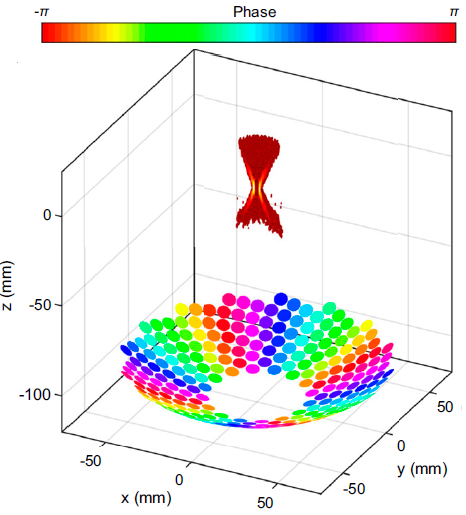
\includegraphics[width=\textwidth]{images/intro/surgery_acTweezer.PNG}
    \caption{}
    \label{fig:ac_tw_surgery}
    \end{subfigure}
    \begin{subfigure}{.58\columnwidth}
    \centering
    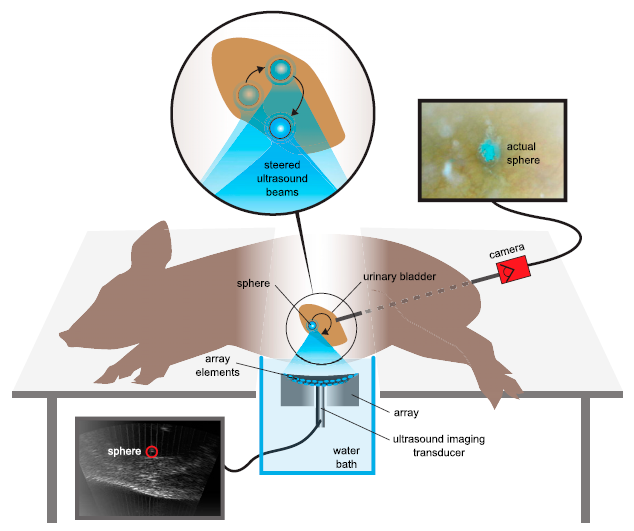
\includegraphics[width=\textwidth]{images/intro/surgery.PNG}
    \caption{}
    \label{fig:pig_surgery}
    \end{subfigure}
    \caption{Focal acoustic tweezer made of an array of transducers to develop surgeries (a), surgery for the extraction of a urinary stone of a pig.}
    \label{fig:pig}
\end{figure}
\section{Previous works}
%ESTADO DEL ARTE

The manipulation of small objects with fields began with the 2018 Nobel Prize study on optical tweezers, developed by Ashkin in 1970, which showed the possibility of trapping and accelerating dielectric particles using the stable potential well of a continuous laser. This result led to the birth of optical tweezers \cite{Ashkin1970}. Parallel to this research, in 1962 the Russian physicist Lev Petrovich Gor'kov, based on King's works on acoustical radiation forces \cite{King1934, King1935}, studied the force exerted by an acoustical field on a spherical particle immersed in an ideal fluid and deduced the so-called Gor'kov potential, which is the basic principle of acoustical tweezers \cite{Gorkov1962}. 
%In Gor'kov's work the force is obtained as the gradient of a multipolar expansion of the velocity potential. 
Further theoretical improvements of the model were done by J. Wu and G. Du in 1990, even proving their results with experiments where  latex particles were confined using two focused PZT transducers \cite{WuDu1990,Wu1991}. Later experiments were carried out to create acoustical traps lab chips to move an array of colloidal particles in the three orthogonal directions of space \cite{Shi2009}. 

%AQUI VOY jdmunozc

Other developments were made of transducer arrays to larger applications like the non-invasive kidney stone expulsion of a pig as seen in figure \ref{fig:pig}. The surgery consisted in manipulating urinary stones to be extracted without making incisions. The surgery was accomplished without damages in the organ tissue, demonstrating the potential of acoustical tweezers for medicine applications \cite{Ghanem2020}. With this potential, micro-robotics has been studied in this field, whether for surgery or drug delivery, as it was proposed by Feynman as "swallowing the surgeon". Self-assembling of micro-beads is the path to develop micro-bots and it's inspired in nature swarms of many biological organisms \cite{Medina2017}. One way to produce clustering or self-assembling uses external rotating magnetic fields, where super-paramagnetic particles are aligned by its magnetic moment forming chains, vortex or ribbons depending on the orientation of controllable external fields. As it is seen from biological organisms like bacteria, spermatozoa, volvox among others particular ways to move and displace through aqueous fluids were viscous forces are dominating (very low Reynolds number), interaction of micro-particles with external fields have become an alternative to produce this kind of "swimming" motion. Many swimming mechanisms are studied from Scallop theorem, however rolling has been considered another motion alternative for micro-bots \cite{Purcell1977,Lauga2010}. The rolling motion has been also observed in nature, as the case of Neutrophil, and its displacement is due to friction with a surface or physical boundary. As micro-beads aggregate into disks or rods to develop rolling and additionally there is a strong dependence on gravity, which is not enough to keep a particle stuck to a wall. Acoustical waves have been used to keep a rolling motion in a surface in order to mimics the rolling motion of Neutrophil. The aggregation of particles to create wheel-like structures has been also carried out to study the dynamics of rolling through a vessel wall to create propulsion using a no-slip boundary condition \cite{Kaiser2017, Xie2019, Han2020,Harting2021,Tasci2015}. 

\begin{figure}[b]
    \begin{subfigure}{.38\columnwidth}
    \centering
    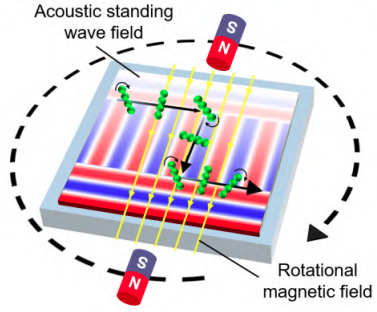
\includegraphics[width=\textwidth]{images/intro/microswimmers_generalScheme.png}
    \caption{}
    \label{fig:ms_gen}
    \end{subfigure}
    \begin{subfigure}{.38\columnwidth}
    \centering
    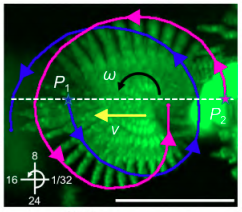
\includegraphics[width=\textwidth]{images/intro/microswimmers_rotation.png}
    \caption{}
    \label{fig:ms_rot}
    \end{subfigure}
    \begin{subfigure}{.8\columnwidth}
    \centering
    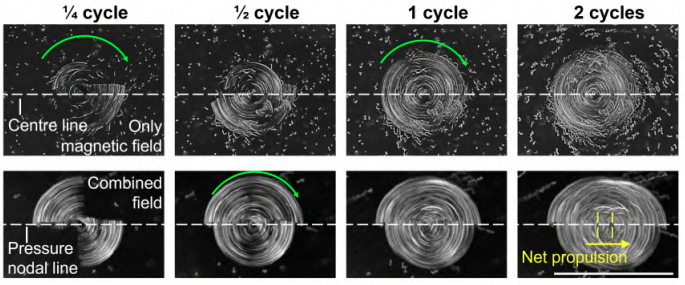
\includegraphics[width=\textwidth]{images/intro/microswimmers_cycles.png}
    \caption{}
    \label{fig:ms_cycles}
    \end{subfigure}
    \caption{General sketch of the rolling Microswimmers experiment (a). Graphical definition of the angular and linear speed of the Microswimmers (b) and comparison of the motion with and without standing waves (c).}
    \label{fig:LBMWaves}
\end{figure}

The rolling motion for chain-shaped microswarms has been studied experimentally by Harting, Malgaretti et. al. to be produced in virtual walls made by standing acoustic waves propagated through the medium \cite{paper_rods}. It is shown that this virtual boundary may be an alternative to develop rolling motion and the spatially asymmetrical hydrodynamic interactions and the help of an external, uniform and rotational magnetic field. The medium is surrounded by piezoelectric transducer which produces the acoustic standing waves along the medium and an acoustic radiation force is made by the particles to be enclosed, assembled into microchains and moving along the nodal plane (see figure \ref{fig:ms_gen}). This may be somehow analogous to the famous experiment of the Chladni patterns, where sand over a vibrating solid plate is being pushed to the nodal planes generated by vibration of the plate. However, this is an experiment taken into the microscopical scale where lengths are in the order of micrometers, the medium is an immerse fluid and instead of ordinary beads, there are microswarms which responds to magnetic fields and can be grouped into clusters instead of being assembled artificially. 
\begin{figure}[t]
    \centering
    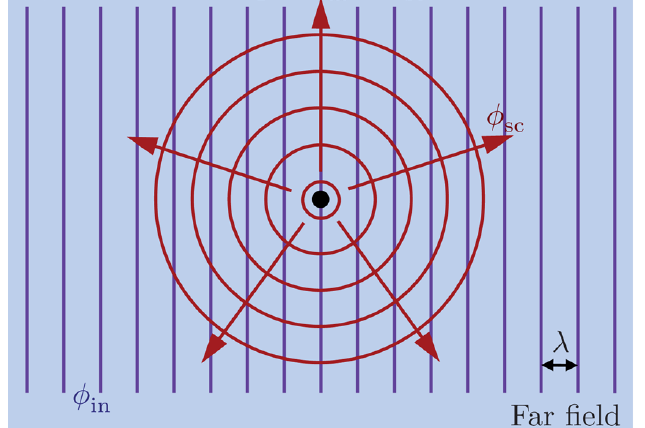
\includegraphics[width=0.45\textwidth]{images/intro/Scattering.PNG}
    \caption{Graphical representation of acoustical scattering where the velocity potential is decomposed into an incident and scattered field.}
    \label{fig:sc_scheme}
\end{figure}
Another key difference is that the acoustic fields may be plane waves guided by the walls in the boundaries instead of being normal modes whose pattern depends on the geometry of the medium and changes drastically with the driven frequency, which makes hard to control the form of the nodal planes. It was shown that the guiding of the nodal planes and the rotating magnetic field make possible the controlling of the motion of the microswarms, as there are linear relationships between the angular frequency of the rotating magnetic field and the linear speed of the microswarms, as well of a proportional relation between the wave's amplitude and the linear speed, shown in fig. \ref{fig:ms_rot}. It was also proved that the influence of the magnetic field by itself does not create a net displacement over the microswarms, therefor, the incident acoustic waves act like virtual boundaries which are useful to guide the movement of the particles as seen in the figure \ref{fig:ms_cycles}. 